\section{Classification}
\label{sec:exp-clf}
    \subsection{Overview}
    \label{subsec:exp-clf-overview}
        In this section, parameters that alter the training set of data-set and those which affect the training process itself will be experimentally optimised to produce near-optimum performance. Due to an exhaustive grid search not being feasible (discussed in section \ref{subsec:bg-intro-structure}), the 'greedy' optimum will be found at each stage, making some assumptions which will then be tested/updated through iteration.
        
        \newcommand{\optnode}[5]{
    % supernode id, find content, assume content, found content, position 
    \node (#1-find) [smallamber,minimum height=0.1cm ,text width=1.6cm,minimum width = 2cm #5] {\specialcell{#2}};
    \node (#1-assume) [smalldarkbyzantium,minimum height=0.1cm, text width=1.6cm, minimum width = 2cm, below=0.15cm of #1-find] {\specialcell{#3}};
    \node (#1-found) [smallazure,minimum height=0.1cm, text width=1.6cm, minimum width = 2cm, below=0.15cm of #1-assume] {\specialcell{#4}};
    \begin{pgfonlayer}{background}
        \node(#1)[bigblush] [fit = (#1-find) (#1-found)] {};
    \end{pgfonlayer}
}
\def\dist{0.3cm}
\begin{tikzfig}{fig:exp-clf-overview-opt}{Optimisation and iteration of pre-classification pipeline.}{\tiny}
    
    \optnode{feats}{choose features}{balance classes\\normalise audio\\training labels\\classifier params}{normalise features\\testing label}{}
    \optnode{balance}{balance classes}{normalise audio\\training labels\\classifier params}{normalise features\\testing label\\chosen features}{, right=\dist of feats-find}
    \optnode{normaud}{normalise audio}{training labels\\classifier params}{normalise features\\testing label\\chosen features\\balance classes}{, right=\dist of balance-find}
    \optnode{labels}{choose train labels}{classifier params}{normalise features\\testing label\\chosen features\\balance classes\\normalise audio}{, right=\dist of normaud-find}
    \optnode{clf}{classifier params}{none}{normalise features\\testing label\\chosen features\\balance classes\\normalise audio\\chosen train labels}{, right=\dist of labels-find}
    \optnode{done}{none}{none}{normalise features\\testing label\\chosen features\\balance classes\\normalise audio\\chosen train labels\\classifier params}{, right=\dist of clf-find}
    
    \optnode{key}{optimising}{assumed}{chosen/estimated}{, left=3cm of balance-find}

    \draw[arrow](feats)--(balance);
    \draw[arrow](balance)--(normaud);
    \draw[arrow](normaud)--(labels);
    \draw[arrow](labels)--(clf);
    \draw[arrow](clf)--(done);
    \draw [arrow] (done-found.east) -| (12.85,-3.37) |- (-1.4,-3.37)  node[near end,above]{iterate}-| (-1.4,-2) |- (feats-assume.west);

    
\end{tikzfig}
        
        Figure \ref{fig:exp-clf-overview-opt} shows how this iterative optimisation takes place, beginning with three assumptions, reasons for which are given in the following sections. Performance will be evaluated using the F1 Score, the area under the ROC curve, the true positive rate (TPR) and the true negative (TNR) rate. These metrics have been chosen as they represent important classifier characteristics in a compact form, convenient for comparing many results. More details regarding metrics can be found in section \ref{sec:pl-test}.
        
    \subsection{Known Parameters}
    \label{subsec:exp-clf-known}
        \subsubsection{Audio Normalisation}
        \label{subsubsec:exp-clf-audio}
            The Culex q. data set used has been recorded using the same device in the same location for each of the 57 recordings, therefore mosquitoes flying into and out of the microphone range will have consistent volumes. Some sections of the recordings contain highly irregular noise that is considerably louder than the mosquitoes, an example noisy signal is shown in \ref{fig:exp-clf-audio-noisy}.
            \begin{figure}[ht]
                \centering
                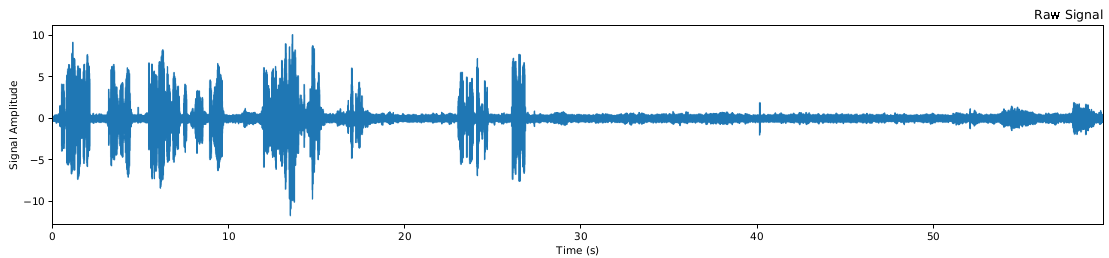
\includegraphics[width=\textwidth]{raw_with_noise}
                \caption{An example of a particularly noisy signal from the Culex. recordings where someone is talking next to the microphone.}
                \label{fig:exp-clf-audio-noisy}
            \end{figure}
            With signals such as these, normalising on a signal-by-signal basis is bad practise for two reasons. Firstly, transforming the signal to unit variance, would significantly shrink the amplitude of the signal in the non-noisy areas, affecting the subsequently generated features and impeding classification ability. Secondly, normalising signal-by-signal over time-dependant is using information that is 'from the future' for classification, leading to unpredictable consequences. The correct way to normalise is to normalise over the whole aggregated training signal then re-using the constants for the aggregated test signal. There is scope for more sophisticated methods of normalisation. For example \textcite{Prabhavalkar2015} have had success using automatic gain control (AGC), improving robustness and performance of speech recognition with deep neural networks. However, significant results in the context of this project are unlikely. This is easier applied in the feature space due to the implementation in MozzPy, detailed in section \ref{subsec:pl-data-software}, so will be left to that stage and not applied here.
            
        \subsubsection{Feature Normalisation}
        \label{subsubsec:exp-clf-featnorm}
            Feature normalisation, or \textit{whitening}, is done with reuse of constants for reasons discussed in above and in section \ref{subsec:pl-data-software}. The impact of normalisation depends on the nature of the classifier being used and how similarity/distance is defined. For a random forest classifier, decisions whether to split a node are based on the information/entropy of the feature (discussed further in \ref{subsec:pl-clf-sup}), a criteria that is invariant to monotonic transforms such as feature scaling \cite{Hastie2009}, so normalisation will not be applied for the random forest.
            
            Linear SVM performance, in comparison, is dependent on feature scaling and normalisation. By not scaling, a feature with larger magnitudes may be assigned a higher importance than one with lower magnitudes. For non-linear kernels, it is dependant on the kernel and how distance/similarity is calculated. Normalisation will be used for the SVM classifier.
            
            Naive Bayes, by design, performs feature scaling when XXXX, \ref{subsec:pl-clf-sup}. 
            
            These conclusions have been confirmed in brief trials where both the random forest and naive Bayes classifiers were unaffected by normalisation, and the SVM was $\sim10$ times slower to train with resultant F1 scores reduced by at least $0.2$.
    
            %[http://stats.stackexchange.com/questions/57010/is-it-essential-to-do-normalization-for-svm-and-random-forest]
         
    \subsection{Assumed Parameters}
    \label{subsec:exp-clf-ass}       
        \subsubsection{Feature Selection}
        \label{subsubsec:exp-clf-ass-featsel}
            use all features because blah
        
        \subsubsection{Label Selection}
            \label{subsubsec:exp-clf-ass-label}
            \begin{wraptable}{r}{0.4\textwidth}
                \scriptsize
                \singlespacing
                \centering
                    \begin{tabular}{ |c|c|c|c| } 
                        \hline
                        \specialcell{No.\\ Disagreements} & 0 & 1 & 2 \\ 
                        \hline
                        \specialcell{Percentage of \\All Labels} & 77.7\% & 16.2\% & 6.04\% \\ 
                        \hline
                    \end{tabular}
                \caption{Disagreement between four people labelling the same data-set.}
                \label{fig:exp-clf-ass-label-agree}
            \end{wraptable}
        
            Analysis of these labels, shown in table \ref{fig:exp-clf-ass-label-agree}, emphasises the difficulty of this problem. Of the four people labelling the data, there is only complete agreement $77\%$ of the time, the rest of the time there is at least one person who disagrees with the others.
        disagreement 77, leaaves enough data to use conf
            justify each assumption eg use conf label bc although less dataa will be better
            then 05 mozz as test label

        \subsubsection{Classifier Parameters}
        \label{subsubsec:exp-clf-ass-param}
            150 trees, rest default
        
    \subsection{Optimisation}
    \label{subsec:exp-clf-opt}
        \subsubsection{Class Balancing}
        \label{subsubsec:exp-clf-opt-class}
            With the known/assumed parameters set, six experiments are carried out and presented in table \ref{fig:exp-clf-opt-class-res}.
            \begin{wraptable}{r}{0.5\textwidth}
                \scriptsize
                \singlespacing
                \centering
                    \begin{tabular}{ |l|c|c|c|c|c| } 
                        \hline
                        Classifier & Balanced & F1 & ROC Area & TPR & FPR \\ 
                        \hline
                        NB & \xmark     &   &   &   & \\
                
                        NB & \checkmark &   &   &   & \\
                 
                        RF & \xmark     &   &   &   & \\
              
                        RF & \checkmark &   &   &   & \\
                 
                        SVM & \xmark     &   &   &   & \\
                    
                        SVM & \checkmark &   &   &   & \\
                        \hline
                    
                    \end{tabular}
                \caption{Results of testing balanced training data against non-balanced.}
                \label{fig:exp-clf-opt-class-res}
            \end{wraptable}
            In all three cases, classifiers with balanced training data outperform those with imbalanced training data. Training examples go from $80024$ and $24695$ for classes 0 and 1 respectively to $24695$ and $24695$. Although overall performance is better, it is interesting to note how balancing classes skews the TPR and TNR to, rather intuitively, increase the former and decrease the latter; a potential technique to tune the classifier. Further experiments will balance the training data to maximise performance.
            
        \subsubsection{Feature Selection}
        \label{subsubsec:exp-clf-opt-featsel}
            Feature design, as detailed in section \ref{sec:pl-feats}, and selection are crucial to any machine learning problem using traditional classifiers. In order to determine which of the audio features to use, twelve tests will be performed per classifier. Ten of the tests will be the classifier trained separately on each feature, the other two will be on a feature set that has been dimensionally reduced, one through recursive feature elimination (RFE) and one through principal component analysis (PCA)., both of which are described in section \ref{subsec:pl-featpreproc-sel} 
            
            RFE
            
            do changing of windows here, say 0.1s res max as that format of lbls
    
        \subsubsection{Label Selection}
        \label{subsubsec:exp-clf-opt-label}
            
        \subsubsection{Classifier Parameters}
        \label{subsubsec:exp-clf-opt-param}
     





%     start with most detail for random forest, then can tell similar story for the other classifiers in less detail
% Sensors]
%     \subsection{Parameters}
%     \label{subsec:exp-rf-param}
%         \begin{sitemize}
%             \item{start with rf because fast and relatively good results, also gives importance of features}
%             \item{choosing number of trees}
%             \item{decision criterion}
            
%             \item{label selection - binary or mc (binary does better)}
%             \item{postprocessing}
%         \end{sitemize}
    
%     \subsection{Feature Processing}
%     \label{subsec:rf-feats}
%         \begin{sitemize}
%             \item{normalisation (built into sklearn implementation?)}
%             \item{feature selection - shows feature importance as well, do pca and rfe and compare, comment on features picked out as important}
%         \end{sitemize}
    
%     \subsection{Label Selection}
%     \label{subsec:rf-labels}
%         \begin{sitemize}
%             \item{show results with all different labels, binary and multiclass, choose best}
%         \end{sitemize}
        
%     \subsection{Post-Processing}
%     \label{subsec:rf-postproc}
%         \begin{sitemize}
%             \item{show how go from fscore of 0.6ish to 0.75ish}
%             \item{show best for each context, in table}
%         \end{sitemize}